\documentclass[11pt,oneside]{scrbook}
\usepackage[pdftex]{graphicx}
\usepackage{url}
\usepackage{html}
\usepackage{notes}
\usepackage{fullpage}

\usepackage[pdftex]{color}
\usepackage{fancybox}
\usepackage{fancyvrb}

\newcommand{\htmldiv}[2]{\HTMLcode[id="#1"]{div}{#2}}

%%
%% COLOR
%%

\definecolor{backgroundgray}{gray}{0.9}

%%
%% FANCYVRB
%%

% Las tabulaciones se substituyen por dos espacios
\fvset{tabsize=2}

% Creamos un nuevo environment de fancyvrb para los ejemplos enmarcados
\DefineVerbatimEnvironment{VerbShell}{BVerbatim}{boxwidth=0.8\textwidth,fontsize=\small,samepage=true,commandchars=\\\{\}}
\DefineVerbatimEnvironment{VerbWideShell}{BVerbatim}{boxwidth=1\textwidth,fontsize=\small,commandchars=\\\{\}}

\newenvironment{shellverbatim}%
{\VerbatimEnvironment\begin{Sbox}\begin{VerbShell}}%
{\end{VerbShell}\end{Sbox}\setlength{\fboxsep}{8pt}\begin{center}\fcolorbox{black}{backgroundgray}{\TheSbox}\end{center}}

\newenvironment{wideshellverbatim}%
{\VerbatimEnvironment\begin{Sbox}\begin{VerbWideShell}}%
{\end{VerbWideShell}\end{Sbox}\setlength{\fboxsep}{8pt}\begin{center}\fcolorbox{black}{backgroundgray}{\TheSbox}\end{center}}

\newenvironment{warning}
{\latexhtml{\begin{importantnote}}{\begin{rawhtml}<div class='warning'>\end{rawhtml}}}
{\latexhtml{\end{importantnote}}{\begin{rawhtml}</div>\end{rawhtml}}}

\setcounter{tocdepth}{1}

\begin{document}
\frontmatter
\title{The Haizea Manual}
\author{Borja Sotomayor}

\begin{latexonly}
\newcommand{\HRule}{\rule{\linewidth}{0.5mm}}

\begin{titlepage}
 
\begin{center}
 
% Title
\HRule \\[0.4cm]

\includegraphics[width=0.6\textwidth]{images/haizea.png}\\[1cm]
\textsc{ \huge The Haizea Manual}\\{\large Technology Preview 1.2}\\{\large 9/29/08}\\[0.4cm]
 
\HRule \\[1.5cm]
\url{http://haizea.cs.uchicago.edu/}

\vfill
 
\begin{flushright} \large
Borja Sotomayor\\
Department of Computer Science\\
University of Chicago\\
\texttt{borja@cs.uchicago.edu}
\end{flushright}
 
\end{center}
 
\end{titlepage}

\end{latexonly}
\begin{htmlonly}
\maketitle
\end{htmlonly}

\tableofcontents

\chapter{Preface}
\section*{What is Haizea?}
\section*{How to read this manual}
\section*{Document conventions}

\mainmatter

\part{Fundamental Concepts}

\chapter{What is Haizea?}
\label{chap:whatis}

Haizea is an open-source VM-based lease management architecture. Let's break that down, shall we?

\begin{description}
\item[Haizea is a resource manager] (or, depending on who you ask, a "resource scheduler"): Haizea is a software component that can manage a set of computers (typically a cluster), allowing users to request exclusive use of those resources described in a variety of terms, such as "I need 10 nodes, each with 1 GB of memory, right now" or "I need 4 nodes, each with 2 CPUs and 2GB of memory, from 2pm to 4pm tomorrow".
\item[Haizea uses leases] The fundamental resource provisioning abstraction in Haizea is the lease. Intuitively, a lease is some form of contract where one party agrees to provide a set of resources (an apartment, a car, etc.) to another party. When a user wants to request computational resources from Haizea, it does so in the form of a lease. When applied to computational resources, the lease abstraction is a powerful and general construct with a lot of nuances. Leases are described in more detail in Chapter~\ref{chap:leases}
\item[Haizea is VM-based] We hold that the best way of implementing resource leases is using virtual machines (VMs). Therefore, Haizea's scheduling algorithms are geared towards managing virtual machines, factoring in all the extra operations (and overhead) involved in managing VMs. The Globus Virtual Workspaces group, where Haizea was originally developed, has an extensive list of publications that argue how using virtual machines for resource leasing is \textsf{A Good Thing} (and also \textsf{Not A Trivial Thing}).
\item[Haizea is open source] Haizea is published under the Apache License 2.0, a BSD-like OSI-compatible license.
\end{description}

\section{What can you do with Haizea?}

Haizea is, primarily, a VM resource management component that takes lease requests and makes scheduling decisions based on those requests, but doesn't actually know anything about how to enact those decisions. For example, Haizea may determine at what times a set of VMs representing a lease must start and stop, but it doesn't actually know how to instruct a virtual machine manager (such as Xen, KVM, etc.) to do these actions. Haizea can, however, delegate these enactment actions to an external component using a simple API. Haizea can currently interface with the OpenNebula (\url{http://www.opennebula.org/}) virtual infrastructure manager to enact its scheduling decisions. Haizea can also simulate enactment actions, which makes it useful for doing scheduling research involving leases or VMs (in fact, the Haizea simulator has been used in a couple of papers).

So, Haizea can be used in three modes: OpenNebula mode, unattended simulation mode, and interactive simulation mode.

\subsection{OpenNebula mode}

\begin{center}
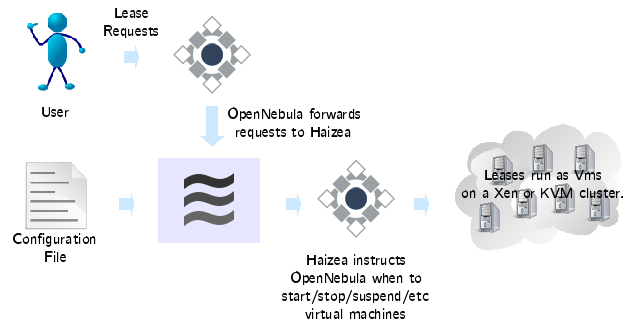
\includegraphics{images/mode_opennebula.png}
\end{center}

Haizea can be used as a drop-in replacement for OpenNebula's scheduling daemon. OpenNebula is a virtual infrastructure manager that enables the dynamic deployment and re-allocation of virtual machines on a pool of physical resources. OpenNebula and Haizea complement each other, since OpenNebula provides all the enactment muscle (OpenNebula can manage Xen and KVM virtual machines on a cluster, with VMWare support to follow shortly) while Haizea provides all the scheduling brains. 

Chapter~\ref{chap:opennebula} describes how to use Haizea and OpenNebula together.

\subsection{Unattended simulation mode}

\begin{center}
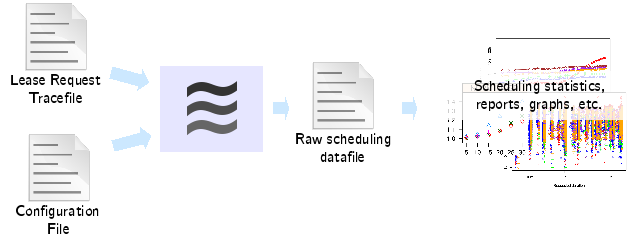
\includegraphics{images/mode_unattended_simulation.png}
\end{center}

In this mode, Haizea takes a list of lease requests (specified in a \emph{tracefile}) and a configuration file specifying simulation and scheduling options (such as the characteristics of the hardware to simulate), and processes them in ``simulated time''. In other words, the goal of this mode is to obtain the final schedule for a set of leases, without having to wait for all those leases to complete in real time (this makes this mode particularly useful to find out what effect a certain scheduling option could have over a period of weeks or months). In fact, the final result of an unattended simulation is a datafile with raw scheduling data and metrics which can be used to generate reports and graphs. 

Chapter~\ref{chap:quickstart} provides a quickstart-style introduction to running Haizea in unattended simulation mode, and Chapter~\ref{chap:simulation} explains simulation options in more detail. Analysis of the scheduling data generated by an unattended simulation is covered in Chapter~\ref{chap:analysing} 

\subsection{Interactive simulation mode}

\begin{center}
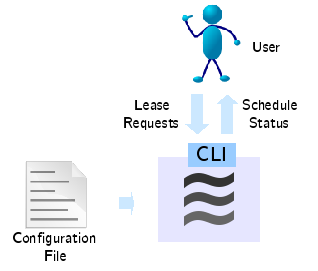
\includegraphics{images/mode_interactive_simulation.png}
\end{center}

In this mode, enactment actions are simulated, but Haizea runs in ``real time''. This means that, instead of having to provide a list of lease requests beforehand, your can use Haizea's command-line interface to request leases interactively and query the status of Haizea's schedule (e.g., to find out the state of lease you've requested). Obviously, this mode is not useful if you want to simulate weeks or months of requests, but it is handy if you want to experiment with leases and track the schedule in a more user-friendly way (since the datafile produced by the unattended simulation is mostly meant for consumption by other programs, e.g., to generate graphs and reports).

Chapter~\ref{chap:quickstart}, the quickstart-style introduction, also includes instructions on how to run Haizea in interactive simulation mode.

\section{Haizea architecture}

\begin{figure}
\begin{center}
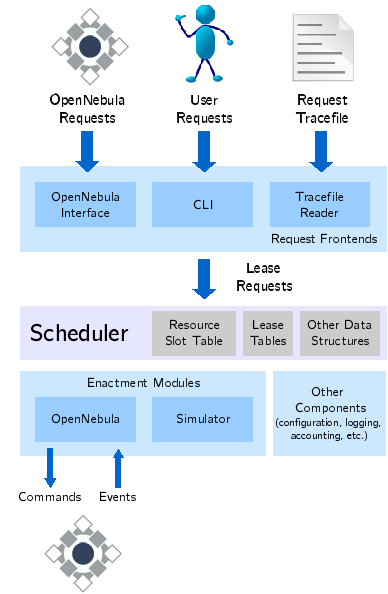
\includegraphics[width=0.4\textwidth]{images/architecture.png}
\end{center}
\caption{The Haizea architecture}
\label{fig:arch}
\end{figure}

The Haizea architecture (see Figure~\ref{fig:arch}) is divided into the following three layers:

\begin{description}
\item[The request frontend] This is where lease requests arrive. Haizea can currently accept requests from OpenNebula, through a command-line interface, or read them from a tracefile (in SWF format or using the Haizea-specific LWF format).
\item[The scheduling core] This is where the lease requests are processed and scheduled, resulting in enactment actions happening at specific points in time (e.g., "Start VM for lease X in node Y at time T", etc.)
\item[The enactment modules] These take care of the "dirty work" of carrying out the enactment actions generated by the scheduler. Haizea can currently send enactment actions to OpenNebula, resulting in Haizea being able to manage Xen and KVM clusters (VMWare support coming soon), or to a simulated cluster.
\end{description}

The Haizea architecture keeps these three layers completely decoupled, which means that adding support for an additional enactment backend only requires writing an enactment module for that backend. The API for enactment modules is still not fully defined, and integration with OpenNebula is currently driving this effort. However, if you'd be interested in using Haizea in another system, please do let us know. We'd be very interested in hearing what your requirements are for the frontend and enactment APIs.

\section{Haizea is still a technology preview}

Haizea started out as research software (and it is still largely meant for research purposes). Although Haizea works and we're getting to the point where it can be used in production systems, it is still a technology preview, so please use it with caution.If you have any trouble using Haizea, or understanding any part of the source code, please don't hesitate to ask for help on our mailing list (see the Haizea website for details on how to subscribe).

\chapter{Resource leases}
\label{chap:leases}
Let's say you need computational resources\ldots

Maybe you're a scientist who needs to run some simulations. You have specific hardware requirements, but you're not particularly picky about when the simulations run, and probably won't even notice if they are interrupted at some point, as long as they finish running (correctly) at some point, maybe before a given deadline. A cluster managed by a job scheduler would probably be a good fit for you.

You could also be a software developer who wants to test his or her code on a pristine machine, which you would only need for a relatively short period of time. Plus, every time you use this machine, you'd like it to start up with the exact same pristine software environment. Oh, and you want your machine now. As in \emph{right now}. One option could be to install a virtual machine (VM) manager (such as Xen, VMWare, etc.) to start up these pristine machines as VMs on your own machine. Even better, you could go to a cloud (like Amazon EC2, \url{http://www.amazon.com/ec2/}, or the Science Clouds, \url{http://workspace.globus.org/clouds/}) and have those VMs appear automagically somewhere else, so you don't have to worry about setting up the VM manager or having a machine powerful enough to run those VMs.

Or perhaps you're a run-of-the-mill geek who wants his or her own web/mail/DNS/etc server. This server will presumably be running for months or even years with high availability: your server has to be running all the time, with no interruptions. There's a whole slew of hosting providers who can give you a dedicated server or a virtual private server. The latter are typically managed with VM-based datacenter managers.

As you can see, there are a lot of resource provisioning scenarios in nature. However, the solutions that have emerged tend to be specific to a particular scenario, to the exclusion of other ones. For example, while job-based systems are exceptionally good at managing complex batch workloads, they're not too good at provisioning resources at specific times (some job-based systems do offer advance reservations, but they have well-known utilization problems) or at giving users unfettered access to provisioned resources (forcing them, instead, to interact with the resources through the job abstraction).

A lease is a general resource provisioning abstraction that could be used to satisfy a variety of use cases, such as the ones described above. In our work, we've defined a lease as a ``negotiated and renegotiable agreement between a resource provider and a resource consumer, where the former agrees to make a set of resource available to the latter, based on a set of lease terms presented by the resource consumer''. In our view, the lease terms must include the following dimensions:

\begin{description}
 \item[Hardware] The hardware resources (CPU, memory, etc.) required by the resource consumer.
 \item[Software] The software environment that must be installed in those resources.
 \item[Availability] The period during which the hardware and software resources must be available. It is important to note that the availability period can be specified in a variety of ways, like ``just get this to me as soon as you can'', ``I need this from 2pm to 4pm on Mondays, Wednesdays, and Fridays (and, if I don't get exactly this, I will be a very unhappy resource consumer)'', or even ``I need four hours sometime before 5pm tomorrow, although if you get the resources to me right now I'll settle for just two hours''. A lease-based system must be able to efficiently combine all these different types of availability.
\end{description}

Furthermore, if you don't get any of these dimensions, then you're being shortchanged by your resource lessor. For example, Amazon EC2 is very good at providing exactly the software environment you want, and reasonably good at providing the hardware you want (although you're limited to a few hardware configurations), but not so good at supporting a variety of availability periods.

So, Haizea aims to support resource leasing along these three dimension. For now, Haizea supports three types of availability:

\begin{description}
\item[Best-effort lease] Resources are provisioned as soon as they are available.
\item[Advance reservation-style leases (or "AR leases")] Resources are provisioned during a strictly defined time period (e.g., from 2pm to 4pm).
\item[Immediate leases] Resources must be provisioned right now, or not at all.
\end{description}

Although there are many systems (particularly job-based systems) that support the first two types of availability, Haizea differs in that it efficiently schedules heterogeneous workloads (combining best-effort and AR leases), overcoming the utilization problems that tend to occur when using ARs. Haizea does this by using virtual machines to implement leases. Virtual machines also enable Haizea to provide exactly the hardware and software requested by the user. Additionally, Haizea also manages the overhead of preparing a lease, to make sure that any deployment operations (such as transferring a VM disk image) are taken care of before the start of a lease, instead of being deducted from the lessee's allocation.

In the future, Haizea will support additional lease types, such as urgent leases, periodic leases, deadline-driven leases, etc.

\section{Supported types of leases}

To better illustrate the types of leases supported in Haizea, let's assume you have a 4-node cluster, and that you want to lease parts of that cluster over time. We'll represent the four nodes over time like this:

\begin{center}
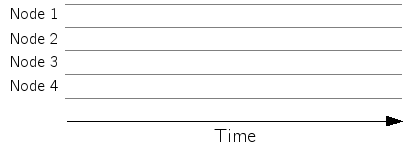
\includegraphics{images/quickstart_leasegraph1.png}
\end{center}

\subsection{``Advance Reservation'' lease}

An advance reservation, or AR, lease is a lease that must begin and end at very specific times. For example, the following lease starts at 1pm and ends at 2pm:

\begin{center}
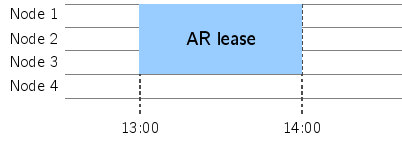
\includegraphics{images/lease_ar.png}
\end{center}

Haizea can schedule this type of lease, which is particularly useful when you need resources at a specific time (for example, to coincide with a lecture, an experiment, etc.)

\subsection{Preemptible best-effort lease}

Sometimes, you know you need resources, but you don't need them at a specific time. In fact, you're perfectly content to wait until there are enough resources available for your lease:

\begin{center}
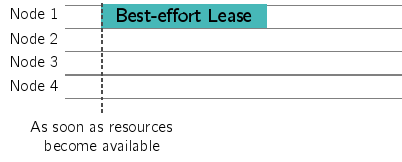
\includegraphics{images/lease_be1.png}
\end{center}


When you request a best-effort lease, your request gets placed in a queue, which is processed in a first-come-first-serve basis (the queue uses backfilling algorithms to improve resource utilization). The downside of this type of lease, of course, is that you may have to wait a while until resources are allocated to your lease:

\begin{center}
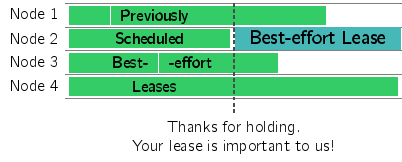
\includegraphics{images/lease_be2.png}
\end{center}

Furthermore, your lease may be running an unattended program which can be safely paused for a while (since no one is interactively using the lease resources). By requesting a preemptible lease, you allow your resources to be preempted by higher-priority leases, like advance reservations:

\begin{center}
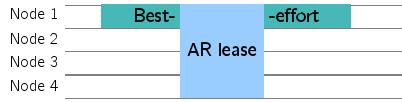
\includegraphics{images/lease_be3.png}
\end{center}

Preemptible best-effort leases are good for running batch jobs, or any non-interactive work. The Haizea paper ``Combining Batch Execution and Leasing Using Virtual Machines'' showed how using the suspend/resume capability of virtual machines allowed AR and best-effort leases to be scheduled together efficiently, overcoming the utilization problems typically associated with ARs.

\subsection{Non-preemptible best-effort lease}

But what if you're willing to wait for your resources to become available, but don't want them to be preempted? (e.g., if you want to use them interactively). Well, it's as simple as requesting a non-preemptible best-effort lease. Once your request makes it through the queue, and your lease is allocated resources, no one is taking them away.

\subsection{Immediate lease}

In some cases, you may need resources now. As in \emph{right now}:

\begin{center}
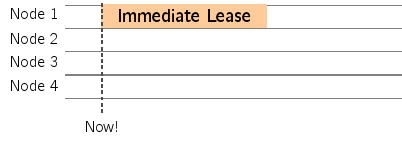
\includegraphics{images/lease_im.png}
\end{center}


Furthermore, if you can't get them right now, you're just not interested in anything else the resource provider has to offer. You're not going to request resources in the future, and you're certainly not going to be put on a queue. This is essentially the type of lease that many cloud systems offer (although the definition of "right now" varies wildly). Take into account that an immediate lease may still take a while to setup (VM image deployment, etc.). This type of lease in Haizea may evolve in the future into an ``urgent lease'', where ``right now'' really does mean ``right now''.

\subsection{Coming soon\ldots}

In the future, Haizea will support more types of leases, such as best-effort leases with deadlines and leases requiring a non-trivial negotiation before the lease is accepted.

\subsubsection{Best-effort with deadlines}

In some cases, when you say ``best effort'', you really mean ``best effort, but be reasonable''. Sure, you're willing to wait for your resources, but you may need them before a deadline.

\begin{center}
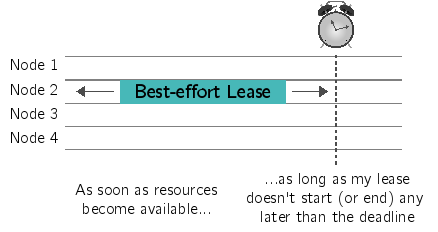
\includegraphics{images/lease_deadline.png}
\end{center}


For example, let's say you want a 16-node cluster sometime today to run a test program. You're not particularly picky about when you get the cluster, as long as it happens today and you're given sufficient warning of when your lease will be available. In the future, you will be able to tell Haizea that you have a deadline, and Haizea will either get the resources to you by then, or tell you that the deadline is simply unfeasible.

\subsubsection{Negotiated leases}

If you've ever entered into any sort of non-computational lease agreement, you know that agreeing on the lease terms rarely involves the lessor instantly being on the same page as you. Rather, it involves a fair amount of haggling. Besides, if your computational needs are flexible, so should your lease manager (c'mon, are you sure you mean "exactly at 2pm"? maybe you meant to say "at some point this afternoon"?). In the future, you will be able to negotiate your leases with Haizea:

\begin{center}
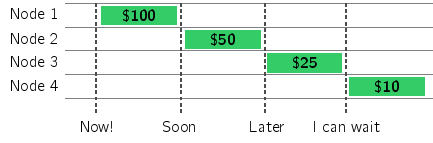
\includegraphics{images/lease_negotiate.png}
\end{center}


So, hey, maybe we can't get you that shiny AR you want at 2pm, but how about I get you twice the resources at an off-peak time? I'll even throw in a discount. And free air conditioning.

\part{Using Haizea}

\chapter{Installing Haizea}
\label{chap:install}
Haizea has been tested only on Unix systems, and these installation instructions are given with a Unix system in mind. However, Haizea includes a small amount of platform-specific code, and should run fine on other systems with minimal effort. If there is enough interest, we can produce installers and installation instructions for other platforms.

Installing Haizea can be accomplished in four simple steps:

\section{Install dependencies}

Haizea has a couple of software dependencies. Let's get them out of the way first:

\begin{itemize}
\item Python 2.5. (\url{http://www.python.org/})
\item mxDateTime 3.1.0 (\url{http://www.egenix.com/products/python/mxBase/mxDateTime/}), part of the eGenix.com mx Base Distribution).
\item Optional: pysqlite (\url{http://oss.itsystementwicklung.de/trac/pysqlite/}). This package is only necessary if you want to use the OpenNebula modules.
\item Optional: Mako Templates for Python 0.2.2 (\url{http://www.makotemplates.org/}). This package is only necessary if you want to automate running multiple simulation experiments (if this doesn't make any sense, you can skip this prerequisite for now; you will be pointed to this prerequisite again in the documentation when you get to running multiple experiments).
\item Optional: Psyco 1.6 (\url{http://psyco.sourceforge.net/}). This package optimizes the execution of Python code, resulting in the simulation code running much faster. You can skip this prerequisite if you are not going to use Haizea to run simulations, or if you are only going to run short simulations.
\end{itemize}

Note that mxDateTime, pysqlite, Mako, and Psyco are all available as packages (DEB, RPM, etc.) on most Linux distributions. If you don't install any of the optional dependencies, Haizea will still run fine, but some functionality may not be available, as noted above.

\section{Download Haizea}

Go to the \htmladdnormallink{download page}{http://haizea.cs.uchicago.edu/download.html} and download the latest version of Haizea. This will be a tarball called \texttt{haizea-XXX.tar.gz}, where XXX will be the version number. For the remainder of the instructions, let's assume that you've saved this file in a directory called \texttt{\$HAIZEA\_INST}.

\section{Install Haizea}

Go into directory \texttt{\$HAIZEA\_INST} and un-tar the installation package:

\begin{shellverbatim}
tar xvzf haizea-XXX.tar.gz
\end{shellverbatim}

This will create a directory called \texttt{haizea-XXX} in \texttt{\$HAIZEA\_INST}. Go into that directory, and as root, run the following:

\begin{shellverbatim}
python setup.py install
\end{shellverbatim}

If you do not have root access, or want to install Haizea in your home directory, run the following:

\begin{shellverbatim}
python setup.py install --home=\$HOME
\end{shellverbatim}

Note: If you have never installed a Python package in your home directory before, make sure you set the environment variable \texttt{PYTHONPATH} appropriately so Python will be aware of the Haizea modules.

\begin{shellverbatim}
export PYTHONPATH=\$HOME/lib/python
\end{shellverbatim}

After running the setup script, you should see a long list of installation and build messages, ending with the following:

\begin{wideshellverbatim}
creating /usr/share/haizea/traces/multi
copying traces/multi/inj1.lwf -> /usr/share/haizea/traces/multi
copying traces/multi/inj2.lwf -> /usr/share/haizea/traces/multi
copying traces/multi/withprematureend.lwf -> /usr/share/haizea/traces/multi
copying traces/multi/withoutprematureend.lwf -> /usr/share/haizea/traces/multi
running install_egg_info
Writing /usr/lib/python2.5/site-packages/haizea-XXX.egg-info
\end{wideshellverbatim}

If you see this, installation has been successful!

\section{Verify installation}

Haizea includes some sample configuration files and lease request tracefiles that you can use to test Haizea. If you installed Haizea as root, you can run the following to test your installation:

\begin{shellverbatim}
haizea -c /usr/share/haizea/etc/sample_trace.conf
\end{shellverbatim}

This will use a sample configuration file to simulate running the scheduler with no requests, resulting in the following (somewhat anticlimactic) output:

\begin{wideshellverbatim}
[2006-11-25 13:00:00.00] TFILE   Loading tracefile /usr/share/haizea/traces/sample.lwf
[2006-11-25 13:00:00.00] TFILE   Loaded workload with 0 requests (0 best-effort + 0 AR)
[2006-11-25 13:00:00.00] RM      Starting resource manager
[2006-11-25 13:00:00.00] CLOCK   Starting simulated clock
[2006-11-25 13:00:00.00] CLOCK   Stopping simulated clock
[2006-11-25 13:00:00.00] RM      Stopping resource manager
[2006-11-25 13:00:00.00] RM        Completed best-effort leases: 0
[2006-11-25 13:00:00.00] RM        Accepted AR leases: 0
[2006-11-25 13:00:00.00] RM        Rejected AR leases: 0
\end{wideshellverbatim}

Ok, not terribly exciting, but if you see this then the basic machinery is working fine. We will see how to do more elaborate simulations, and how to use Haizea to manage real hardware, in the next chapters.

Note: If you installed Haizea in your home directory, you will have to run the following:

\begin{shellverbatim}
haizea -c \$HOME/share/haizea/etc/sample.conf
\end{shellverbatim}

Additionally, you will have to modify the tracefile option in the sample configuration so it will point to the sample tracefile located in \texttt{\$HOME/share/haizea/traces/sample.lwf} (instead of under the \texttt{/usr} directory).

\chapter{Quickstart guide}
\label{chap:quickstart}
This chapter provides a quick hands-on introduction to using Haizea in simulation mode. Even if you intend to use Haizea in combination with another system, such as OpenNebula, you may still find this guide useful to familiarise yourself with the Haizea configuration file and command-line interface. This chapter assumes that Haizea is installed on your system. If you have arrived at this chapter directly, you may want to read Chapter~\ref{chap:whatis} (``What is Haizea?'') first, although you should still be able to follow the instructions in this chapter without reading Chapter~\ref{chap:whatis} first.

\section{The \texttt{haizea} command}

The main command in the Haizea system is, unsurprisingly, the \texttt{haizea} command. Running this command starts up the Haizea lease manager, which is then ready to receive and schedule lease requests. As described in Chapter~\ref{chap:whatis}, Haizea can run in one of three modes: unattended simulated mode, interactive simulated mode, and OpenNebula mode. In this chapter we will focus on the simulation modes, starting with the ``unattended'' variety. Both simulation modes, and the OpenNebula mode, will be described in more detail in the next chapters.

When running Haizea in unattended simulation mode, the inputs to Haizea are going to be the following:

\begin{description}
 \item [The Haizea configuration file:] A text file containing all the options
 \item [A request \emph{tracefile}:] A text file containing a list of lease requests. Since we are using ``simulated time'', we won't be able to use Haizea interactively (we will be able to do this when we switch to the ``real time'' mode later in the chapter). Instead, we need to provide all the lease requests beforehand.
\end{description}

Based on the configuration file and the lease requests, the simulator produces a schedule for those leases, which you will be able to follow through logging messages printed by Haizea. At the end of the simulation, Haizea also saves a fair amount of raw data and statistics to disk which can be used to produce reports and graphs (a module to do this for you is in the works). This particular mode, with simulated time, is particularly useful when you want to take a list of request (potentially spanning weeks or months) to see what happens when you tweak the scheduling options (without having to wait weeks or months for the result).

So, let's start by writing a configuration file specifying the simulation options (e.g., the characteristics of the simulated cluster) and the scheduling options.

\section{The configuration file}

A sample configuration file is provided with Haizea and is located in \texttt{/usr/share/haizea/etc/sample\_trace.conf} (or \texttt{\$HOME/share/haizea/etc/sample\_trace.conf} if you installed Haizea in your home directory). For this guide, you may want to make a copy of this file and use that instead (so you can preserve the original sample file). If you look at the contents of the file, you will see that it also includes documentation on every option. For now, take a look at the following three options:

\begin{wideshellverbatim}
[simulation]
starttime: 2006-11-25 13:00:00
resources: 4  CPU:100 Memory:1024
\end{wideshellverbatim}

These options are used to describe the characteristics of our simulated cluster. In particular, we're using a 4-node cluster, each node with 1 CPU, 1024 MB of memory. In this document, we will represent this cluster over time like this:

\begin{center}
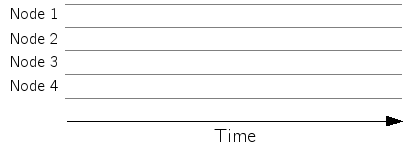
\includegraphics{images/quickstart_leasegraph1.png}
\end{center}

For example, the following figure shows a lease scheduled on Node 1 from 13:00 to 14:00:

\begin{center}
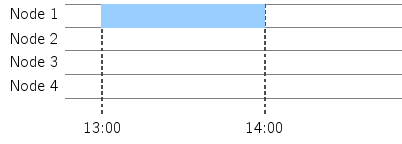
\includegraphics{images/quickstart_leasegraph2.png}
\end{center}

The \texttt{starttime} option is used to specify the time at which the simulated clock should start. As you will see, the configuration file has an abundance of other options. We will cover some of them in this chapter, but a more complete reference can be found in Appendix~\ref{app:conffile}.

\section{The tracefile}

As mentioned earlier, the simulator will read trace requests from a tracefile. The location of this tracefile is specified in the configuration file, in the \texttt{[tracefile]} section:

\begin{wideshellverbatim}
[tracefile]
tracefile: /usr/share/haizea/traces/sample.lwf 
\end{wideshellverbatim}

The default value is a sample tracefile included with Haizea. If you copy the file to a different location, make sure to update the \texttt{tracefile} option accordingly. The format of this file is LWF (Lease Workload Format), an XML format which is particular to Haizea. For now, don't worry about parsing the trace format in detail; it is fairly human-readable and you can also find details on the LWF format in Appendix~\ref{app:lwf}.

\begin{wideshellverbatim}
<lease-workload name="sample">
	<description>
	A simple trace where an AR lease preempts a 
	best-effort lease that is already running. 
	</description>

	<lease-requests>
	
	<!-- The lease requests are initially commented out -->
	
	<!-- First lease request -->
	<!--
	...
	-->

	<!-- Second lease request -->
	<!--
	...
	-->
	
	</lease-requests>
</lease-workload>
\end{wideshellverbatim}

As you can see, there are two lease requests in the file, but they are initially commented out. We will take a closer look at each of these requests next.

\section{Running the simulator}

Now that we have a configuration file and a tracefile, we can run the simulator. You can run Haizea with the sample configuration file like this:

\begin{shellverbatim}
haizea -c /usr/share/haizea/etc/sample_trace.conf 
\end{shellverbatim}

Which results in the following output:

\begin{wideshellverbatim}
[2006-11-25 13:00:00.00] TFILE   Loading tracefile /usr/share/haizea/traces/sample.lwf
[2006-11-25 13:00:00.00] TFILE   Loaded workload with 0 requests ()
[2006-11-25 13:00:00.00] RM      Starting resource manager
[2006-11-25 13:00:00.00] CLOCK   Starting simulated clock
[2006-11-25 13:00:00.00] CLOCK   Simulated clock has stopped
[2006-11-25 13:00:00.00] RM      Stopping resource manager gracefully...
[2006-11-25 13:00:00.00] RM      --- Haizea status summary ---
[2006-11-25 13:00:00.00] RM      Number of leases (not including completed): 0
[2006-11-25 13:00:00.00] RM      Completed leases: 0
[2006-11-25 13:00:00.00] RM      Completed best-effort leases: 0
[2006-11-25 13:00:00.00] RM      Queue size: 0
[2006-11-25 13:00:00.00] RM      Accepted AR leases: 0
[2006-11-25 13:00:00.00] RM      Rejected AR leases: 0
[2006-11-25 13:00:00.00] RM      Accepted IM leases: 0
[2006-11-25 13:00:00.00] RM      Rejected IM leases: 0
[2006-11-25 13:00:00.00] RM      ---- End summary ----
\end{wideshellverbatim}

Now that you've seen the tracefile, you can see why the simulator starts up and immediately stops: all the lease requests in the tracefile are commented out, and there's nothing to schedule. Go ahead and uncomment the first lease request, which looks like this:

\begin{wideshellverbatim}
<lease-request arrival="00:00:00">
<lease preemptible="true">
	<nodes>
		<node-set numnodes="1">
			<res type="CPU" amount="100"/>
			<res type="Memory" amount="1024"/>
		</node-set>
	</nodes>	
	<start></start>
	<duration time="01:00:00"/>
	<software>
		<disk-image id="foobar.img" size="1024"/>
	</software>
</lease>
</lease-request>
\end{wideshellverbatim}

This is a request for a best-effort lease (notice how the starting time is left empty, meaning it's up to Haizea to determine the start time), requested at time 00:00:00 (right at the start of the simulation), requiring 1 hour, and only one node. Now run Haizea again. You should now see the following:

\begin{wideshellverbatim}
[2006-11-25 13:00:00.00] TFILE   Loading tracefile /usr/share/haizea/traces/sample.lwf
[2006-11-25 13:00:00.00] TFILE   Loaded workload with 1 requests (1 Best-effort)
[2006-11-25 13:00:00.00] RM      Starting resource manager
[2006-11-25 13:00:00.00] CLOCK   Starting simulated clock
[2006-11-25 13:00:00.00] LSCHED  Lease #1 has been requested.
[2006-11-25 13:00:00.00] LSCHED  Lease #1 has been marked as pending.
[2006-11-25 13:00:00.00] LSCHED  Queued best-effort lease request #1, 1 nodes for 01:00:00.00.
[2006-11-25 13:00:00.00] LSCHED  Next request in the queue is lease 1. Attempting to schedule...
[2006-11-25 13:00:00.00] VMSCHED Lease #1 has been scheduled on nodes [1] 
                                 from 2006-11-25 13:00:00.00 
                                   to 2006-11-25 14:00:00.00
[2006-11-25 13:00:00.00] VMSCHED Started VMs for lease 1 on nodes [1]
[2006-11-25 14:00:00.00] VMSCHED Stopped VMs for lease 1 on nodes [1]
[2006-11-25 14:00:00.00] VMSCHED Lease 1's VMs have shutdown.
[2006-11-25 14:00:00.00] CLOCK   Simulated clock has stopped
[2006-11-25 14:00:00.00] RM      Stopping resource manager gracefully...
[2006-11-25 14:00:00.00] RM      --- Haizea status summary ---
[2006-11-25 14:00:00.00] RM      Number of leases (not including completed): 0
[2006-11-25 14:00:00.00] RM      Completed leases: 1
[2006-11-25 14:00:00.00] RM      Completed best-effort leases: 1
[2006-11-25 14:00:00.00] RM      Queue size: 0
[2006-11-25 14:00:00.00] RM      Accepted AR leases: 0
[2006-11-25 14:00:00.00] RM      Rejected AR leases: 0
[2006-11-25 14:00:00.00] RM      Accepted IM leases: 0
[2006-11-25 14:00:00.00] RM      Rejected IM leases: 0
[2006-11-25 14:00:00.00] RM      ---- End summary ----
\end{wideshellverbatim}

The above corresponds to the following schedule:

\begin{center}
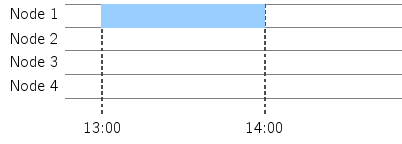
\includegraphics{images/quickstart_leasegraph2.png}
\end{center}

A best-effort request is received at 13:00 and, since the cluster is empty, it is scheduled immediately. Notice how the VMs for the lease start at 13:00 and stop at 14:00. For now, we're assuming that the disk images are predeployed on the physical nodes (we will modify this option in the next section).

Now go ahead and uncomment the second lease request, which looks like this:

\begin{wideshellverbatim}
<lease-request arrival="00:15:00">
<lease preemptible="false">
	<nodes>
		<node-set numnodes="4">
			<res type="CPU" amount="100"/>
			<res type="Memory" amount="1024"/>
		</node-set>
	</nodes>
	<start>
		<exact time="00:30:00"/>
	</start>
	<duration time="00:30:00"/>
	<software>
		<disk-image id="foobar.img" size="1024"/>
	</software>
</lease>
</lease-request>
\end{wideshellverbatim}

This is a request for an advance reservation lease (notice how there is an exact starting time specified), requesting all four nodes for 30 minutes. So, what would happen if we also added this AR lease? Since it requires all the cluster resources from 13:30 to 14:00, the best-effort lease will be unable to run in that time interval. Since the leases are implemented as VMs, Haizea will still schedule the best-effort lease to start at 13:00, but will suspend it before the AR lease starts, and will resume it once the AR lease has finished. In effect, we want the schedule to look like this:

\begin{center}
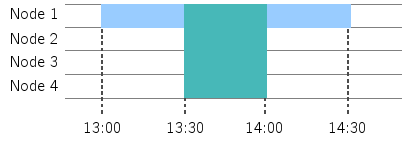
\includegraphics{images/quickstart_leasegraph3.png}
\end{center}

Uncomment the AR lease request, and run Haizea again. You should now see the following:

\begin{wideshellverbatim}
[2006-11-25 13:00:00.00] TFILE   Loading tracefile /usr/share/haizea/traces/sample.lwf
[2006-11-25 13:00:00.00] TFILE   Loaded workload with 2 requests (1 Best-effort + 1 AR)
[2006-11-25 13:00:00.00] RM      Starting resource manager
[2006-11-25 13:00:00.00] CLOCK   Starting simulated clock
[2006-11-25 13:00:00.00] LSCHED  Lease #1 has been requested.
[2006-11-25 13:00:00.00] LSCHED  Lease #1 has been marked as pending.
[2006-11-25 13:00:00.00] LSCHED  Queued best-effort lease request #1, 1 nodes for 01:00:00.00.
[2006-11-25 13:00:00.00] LSCHED  Next request in the queue is lease 1. Attempting to schedule...
[2006-11-25 13:00:00.00] VMSCHED Lease #1 has been scheduled on nodes [1] 
                                 from 2006-11-25 13:00:00.00 
                                   to 2006-11-25 14:00:00.00
[2006-11-25 13:00:00.00] VMSCHED Started VMs for lease 1 on nodes [1]

[2006-11-25 13:15:00.00] LSCHED  Lease #2 has been requested.
[2006-11-25 13:15:00.00] LSCHED  Lease #2 has been marked as pending.
[2006-11-25 13:15:00.00] LSCHED  Scheduling AR lease #2, 4 nodes
                                 from 2006-11-25 13:30:00.00 
                                   to 2006-11-25 14:00:00.00.
[2006-11-25 13:15:00.00] LSCHED  Must preempt leases [1] to make room for lease #2
[2006-11-25 13:15:00.00] LSCHED  Preempting lease #1...
[2006-11-25 13:15:00.00] LSCHED  ... lease #1 will be suspended 
                                     at 2006-11-25 13:30:00.00.
[2006-11-25 13:15:00.00] LSCHED  AR lease #2 has been scheduled.

[2006-11-25 13:29:28.00] VMSCHED Stopped VMs for lease 1 on nodes [1]
[2006-11-25 13:29:28.00] VMSCHED Suspending lease 1...

[2006-11-25 13:30:00.00] VMSCHED Lease 1 suspended.
[2006-11-25 13:30:00.00] VMSCHED Started VMs for lease 2 on nodes [2, 3, 4, 1]
[2006-11-25 13:30:00.00] LSCHED  Next request in the queue is lease 1. Attempting to schedule...
[2006-11-25 13:30:00.00] VMSCHED Lease #1 has been scheduled on nodes [1]
                                 from 2006-11-25 14:00:00.00 (resuming) 
                                   to 2006-11-25 14:31:04.00

[2006-11-25 14:00:00.00] VMSCHED Stopped VMs for lease 2 on nodes [2, 3, 4, 1]
[2006-11-25 14:00:00.00] VMSCHED Resuming lease 1...
[2006-11-25 14:00:00.00] VMSCHED Lease 2's VMs have shutdown.

[2006-11-25 14:00:32.00] VMSCHED Resumed lease 1
[2006-11-25 14:00:32.00] VMSCHED Started VMs for lease 1 on nodes [1]

[2006-11-25 14:31:04.00] VMSCHED Stopped VMs for lease 1 on nodes [1]
[2006-11-25 14:31:04.00] VMSCHED Lease 1's VMs have shutdown.
[2006-11-25 14:31:04.00] CLOCK   Simulated clock has stopped
[2006-11-25 14:31:04.00] RM      Stopping resource manager gracefully...
\end{wideshellverbatim}

Notice how the above corresponds to the previous figure. In particular, notice the following:

\begin{itemize}
 \item  When the AR lease request is received, Haizea looks at the schedule and determines that the only way to schedule the AR lease is to preempt the best-effort lease. However, instead of cancelling that lease, it will just reschedule it so it is suspended right before the AR lease start. Note that Haizea will always try to minimise the number of preemption (in this case, we're forcing the situation for demonstration purposes) by assigning the AR lease to resources that are available without preempting other leases.
 \item Shortly before the AR lease starts, the best-effort lease is suspended (the time required to do this is estimated by Haizea based on an option in the configuration file). When the AR lease ends at 14:00, Haizea begins resuming the suspended best-effort lease.
\end{itemize}

\section{The scheduling options}

Haizea has several scheduling options that control how Haizea selects resources and schedules leases. For example, the above example assumed that leases can be suspended (which they generally always can be when running as virtual machines). What would happen if this were not possible? You can modify the suspension option in the \texttt{[scheduling]} section to find out:

\begin{wideshellverbatim}
[scheduling]
...

suspension: none

...
\end{wideshellverbatim}

Rerun Haizea. Now, when the AR lease arrives at 13:15, the scheduler will realise it has to preempt the best-effort lease to make room for the AR lease, but will no longer be able to suspend it. The only option is to cancel the best-effort lease and resubmit it to the queue:

\begin{wideshellverbatim}
[2006-11-25 13:15:00.00] LSCHED  Preempting lease #1...
[2006-11-25 13:15:00.00] LSCHED  ... lease #1 has been cancelled and requeued
\end{wideshellverbatim}

Now, the best-effort lease can only be scheduled after the AR lease, at 14:00:

\begin{wideshellverbatim}
[2006-11-25 13:15:00.00] VMSCHED Lease #1 has been scheduled on nodes [1] 
                                 from 2006-11-25 14:00:00.00 
                                   to 2006-11-25 15:00:00.00
\end{wideshellverbatim}

So, the schedule would end up looking like this:

\begin{center}
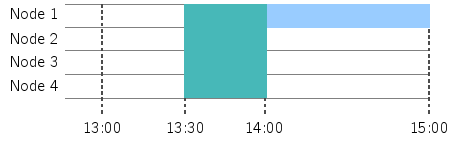
\includegraphics{images/quickstart_leasegraph4.png}
\end{center}

Notice how, although suspending a lease is a disruptive activity which can delay the completion time of a best-effort request, it is still much better than completely cancelling a request and waiting for enough resources to accommodate the entire (uninterrupted) duration of the lease.

Another scheduling option you can modify is whether Haizea should transfer the VM's disk image from an image repository before the lease can start. You can do this by modifying the \texttt{lease-deployment} option:

\begin{wideshellverbatim}
[general]
...
lease-preparation: imagetransfer
...
\end{wideshellverbatim}

If you look at the bottom of the sample configuration file, you will find a section called \texttt{[deploy-imagetransfer]} with all the image transfer options.

Rerun Haizea again. You should get a schedule similar to the previous one, but with some extra messages indicating that image transfers are taking place:

\begin{wideshellverbatim}
[2006-11-25 13:00:00.00] DEPLOY  Starting image transfer for lease 1
[2006-11-25 13:01:22.00] DEPLOY  Completed image transfer for lease 1
\end{wideshellverbatim}

As you can see, the best-effort lease can no longer start right at 13:00, since an image transfer has to take place before the starting time. The same is true of the AR lease, but notice how Haizea schedules the image transfer in such a way that the AR lease can still start at 13:30 as planned (instead of delaying the starting time until 13:31:22).

There are several other options you can modify in the \texttt{[scheduling]} section, such as what backfilling algorithm to use, whether to allow lease migration or not, etc. These options are described in the following chapters, and in Appendix~\ref{app:conffile}.

\section{Interactive simulations} 

Up to this point, Haizea has been scheduling leases in ``simulated time''. This meant that we provided Haizea with a lease workload beforehand, ran it, and got the results of scheduling that workload much earlier than it would have actually taken to run the leases (e.g., if we requested a 30 minute lease, we didn't have to wait 30 minutes for the lease to complete; Haizea just skipped from the start to the end of the lease). This ``fast forward'' approach is useful if you want to experiment with different scheduling parameters and workloads. However, you can also run Haizea in simulation and in ``real time''. To do this, you need to change the \texttt{clock} option of the \texttt{[simulation]} section:

\begin{wideshellverbatim}
[simulation]
...
clock: real
...
\end{wideshellverbatim}

If you run Haizea in this mode, it will run a daemon that is ready to accept your requests interactively through a command-line interface, instead of processing a list of requests provided beforehand. You should see the following when running the \texttt{haizea} command:

\begin{wideshellverbatim}
Started Haizea daemon with pid NNNN
\end{wideshellverbatim}

You will then get control of your console back. If you're wondering where all the logging messages are being saved to, they're now being sent to a file. The default logfile is \texttt{/var/tmp/haizea.log}. You can take a peek at it like this:

\begin{shellverbatim}
tail /var/tmp/haizea.log
\end{shellverbatim}

You will notice messages like this:

\begin{wideshellverbatim}
[2008-09-24 14:14:18.58] CLOCK   Going back to sleep. 
                                 Waking up at 2008-09-24 14:15:19.00 
                                 to see if something interesting has 
                                 happened by then.
\end{wideshellverbatim}

Since time is not simulated, Haizea doesn't know what the ``next time'' to skip to will be, so it will simply wake up periodically to see if anything interesting has happened (like a new request). This interval can be changed in the configuration file:

\begin{wideshellverbatim}
[simulation]
...
wakeup-interval: 10
...
\end{wideshellverbatim}

However, when Haizea plans an event (e.g., leases that have to start or end), it will wake up specifically to handle that event (instead of waiting for the wakeup interval to conclude).

So, let's give Haizea something to do. The \texttt{haizea-request-lease} command is used to request leases. For example, the following command is used to request an 1-node AR lease one minute in the future, for ten minutes:

\begin{wideshellverbatim}
haizea-request-lease -t +00:02:00 -d 00:10:00 -n 1 --non-preemptible \
                     -c 1 -m 512 -i foobar.img -z 600 
\end{wideshellverbatim}

Additionally, you can also write a lease request using the XML format seen previous, save it to a file, and have \texttt{haizea-request-lease} command parse it:

\begin{wideshellverbatim}
haizea-request-lease -f request.xml
\end{wideshellverbatim}

You can find more details on this command's parameters by running \texttt{haizea-request-lease -h} or taking a look at Appendix~\ref{app:cli}. Once you've submitted the lease, you should see the following:

\begin{wideshellverbatim}
Lease submitted correctly.
Lease ID: 1
\end{wideshellverbatim}

You can check the status of your submitted lease by looking at the log file or, more conveniently, using this command:

\begin{shellverbatim}
haizea-list-leases
\end{shellverbatim}

You should see the following:

\begin{wideshellverbatim}
 ID   Type          State      Starting time           Duration      Nodes  
 1    AR            Scheduled  2009-08-04 11:25:57.00  00:10:00.00   1        
\end{wideshellverbatim}

Note: You may not see your lease right away, since Haizea has to ``become aware'' of it (which won't happen until it wakes up to check if there are any new requests). Future versions of Haizea will enable it to be notified immediately of incoming requests.

Remember that the lease has been requested one minute into the future, so it will remain in a ``Scheduled'' state for a couple seconds. If you run \texttt{haizea-list-leases} periodically, you should see it pass through a couple other states. If image transfers are still enabled, it will first transition to the ``Preparing'' state:

\begin{wideshellverbatim}
 ID   Type          State      Starting time           Duration      Nodes  
 1    AR            Preparing  2009-08-04 11:25:57.00  00:10:00.00   1       
\end{wideshellverbatim}

And then to the ``Active'' state:

\begin{wideshellverbatim}
 ID   Type          State      Starting time           Duration      Nodes  
 1    AR            Active     2009-08-04 11:25:57.00  00:10:00.00   1       
\end{wideshellverbatim}

Now let's request a best-effort lease:

\begin{wideshellverbatim}
haizea-request-lease -t best_effort -d 00:10:00 -n 4 --non-preemptible \
                     -c 1 -m 512 -i foobar.img -z 600
\end{wideshellverbatim}

The list of leases will now look like this:

\begin{wideshellverbatim}
 ID   Type          State      Starting time           Duration      Nodes  
 1    AR            Active     2009-08-04 11:25:57.00  00:10:00.00   1       
 2    Best-effort   Scheduled  Unspecified             00:10:00.00   4       
\end{wideshellverbatim}

Note how, for best-effort leases, the starting time is set to ``Unspecified'', which means this time is not specified by the user, but instead determined on a best-effort basis by the scheduler. Since the lease is in a ``Scheduled'' state, that means that it has been assigned a starting time (although that information is currently not available through the command-line interface; it can be seen in the Haizea log).

Now try to rerun the \texttt{haizea-request-lease} command a couple times (i.e., lets submit a couple more best-effort requests). The scheduler won't be able to schedule them, since they require all the available nodes, and the AR lease is using up one of them. The previous best-effort lease was scheduled because Haizea's default behaviour is to schedule at most one best-effort lease in the future if resources cannot be found right away (this is due to Haizea's use of backfilling algorithms; for now, don't worry if you don't know what they are). Anyway, the list of leases should now look like this:

\begin{wideshellverbatim}
 ID   Type  State      Starting time           Duration      Nodes  
 1    AR            Active     2009-08-04 11:25:57.00  00:10:00.00   1       
 2    Best-effort   Scheduled  Unspecified             00:10:00.00   4       
 3    Best-effort   Queued     Unspecified             00:10:00.00   4       
 4    Best-effort   Queued     Unspecified             00:10:00.00   4       
 5    Best-effort   Queued     Unspecified             00:10:00.00   4       
 6    Best-effort   Queued     Unspecified             00:10:00.00   4       
\end{wideshellverbatim}

Notice how the extra best-effort requests have been queued. If you only want to see the contents of the queue, you can use the following command:

\begin{shellverbatim}
haizea-show-queue
\end{shellverbatim}

This should show the following:

\begin{wideshellverbatim}
 ID   Type          State      Starting time           Duration      Nodes  
 3    Best-effort   Queued     Unspecified             00:10:00.00   4       
 4    Best-effort   Queued     Unspecified             00:10:00.00   4       
 5    Best-effort   Queued     Unspecified             00:10:00.00   4       
 6    Best-effort   Queued     Unspecified             00:10:00.00   4       
\end{wideshellverbatim}

When you're done, you can shut Haizea down cleanly by running the following:

\begin{shellverbatim}
haizea --stop
\end{shellverbatim}


\section{Other things you can do with Haizea}

At this point, we have seen how to run simple simulations with Haizea. However, there is a lot more that Haizea can do:

\begin{description}
\item[Run on real hardware] First and foremost, almost everything you just saw above in simulation can be done on real hardware. This is accomplished by using Haizea with the OpenNebula virtual infrastructure manager. So, if you have a Xen or KVM cluster, you can just install OpenNebula and Haizea to enable your users to request VM-based leases on your cluster. This is explained in Chapter~\ref{chap:opennebula}.
\item[Run complex simulations] This chapter concerned itself mostly with scheduling two leases on a 4-node cluster during a span of roughly 2 hours. \emph{Boring}. Haizea can handle more complex simulations, and also provides the necessary tools for you to easily run multiple simulations with different profiles. For example, in the Haizea paper ``Combining Batch Execution and Leasing Using Virtual Machines'' (see the Haizea publication page: \url{http://haizea.cs.uchicago.edu/pubs.html}) we simulated running 72 30-day workloads in six different configurations, or 36 years of lease scheduling. Running multiple simulations is explained in Section~\ref{sec:multiplesim}
\item[Produce reports and graphs] The above examples relied on reading the Haizea log messages or peeking into Haizea's schedule using command-line tools. This is ok for a simple simulation, but no fun when you're scheduling thousands of leases. Haizea saves a fair amount of raw data to disk with scheduling metrics, utilization information, etc. which can be used to generate reports and graphs. We are in the process of producing tools that will allow you to easily analyse that data and create graphs, although some pointers on how to interpret the raw data produced by Haizea are presented in Chapter~\ref{chap:analysing}.
\end{description}

\chapter{Running scheduling simulations}
\label{chap:opennebula}
This chapter describes how to run Haizea in simulation mode. Since the Quickstart Guide (Chapter~\ref{chap:quickstart}) already provides a tutorial-like introduction to running simulations, this chapter is meant mostly as a reference guide, and covers the main simulation and scheduling options. However, it does not cover \emph{all} possible options in the configuration file (a description of all options and their valid values can be found in Appendix~\ref{app:conffile}). It also refers to scheduling algorithms that are not currently explained in the manual (they are described in some of the Haizea scientific publications, but these might be hard to swallow). Future versions of the Haizea manual will include a description of the main scheduling algorithms used, to better orient your choice of scheduling options. Finally, this chapter also covers how to run multiple unattended simulations.

\section{Unattended simulations}

To run Haizea as an unattended simulation requires setting the following options in the configuration file:

\begin{wideshellverbatim}
[general]
...
mode: simulated
...

[simulation]
...
clock: simulated
...
\end{wideshellverbatim}

Additionally, the starting time of the simulation must be specified, along with a stopping condition:

\begin{wideshellverbatim}
[simulation]
...
starttime: 2006-11-25 13:00:00
stop-when: all-leases-done | 
           besteffort-submitted |
           besteffort-done
...
\end{wideshellverbatim}


\section{Interactive simulations}

To run Haizea as an interactive simulation, the following options must be set in the configuration file:

\begin{wideshellverbatim}
[general]
...
mode: simulated
...

[simulation]
...
clock: real
...
\end{wideshellverbatim}


\section{Specifying the simulated physical resources}

The simulated physical resources are specified using the \texttt{resources} option in the \texttt{[simulation]} section. This option can take two values, "in-tracefile", which means that the description of the simulated site is in the tracefile, or a string specifying the site's resources. For the former, see Appendix~\ref{app:lwf} for details on how the simulated site is specified in the tracefile. When using the latter, the format of the string is:

\begin{wideshellverbatim}
<numnodes> <resource_type>:<resource_quantity>[,<resource_type>:<resource_quantity>]*
\end{wideshellverbatim}
 
For example:

\begin{wideshellverbatim}
[simulation]
...
resources: 4  CPU:100 Memory:1024
...
\end{wideshellverbatim}

The above describes a site with four nodes, each with one CPU and 1024 MB of memory. Note that you must always specify at least the ``CPU'' and ``Memory'' resource types.

\section{Scheduling options}

The scheduling options control how leases are assigned to resources.

\subsection{Scheduling policies}

Haizea includes a policy decision module that supports ``pluggable policies'', allowing developers to write their own scheduling policies. This is described in more detail in Chapter~\ref{chap:policies}, and we describe here only the built-in policies that are included with Haizea.

The first policy is lease admission, which controls what leases are accepted by Haizea. Take into account that this decision takes place before Haizea even attempts to schedule the lease (so, you can think of lease admission as ``eligibility to be scheduled''). The two built-in policies are to accept all leases, and to accept all leases \emph{except} advance reservations.

\begin{wideshellverbatim}
[scheduling]
...
policy-admission: accept-all | no-ARs | <custom policy>
...
\end{wideshellverbatim}

The next policy is lease preemptability, or what leases can be preempted. The two built-in policies are to not allow any preemptions, and to allow all ARs to preempt other leases.

\begin{wideshellverbatim}
[scheduling]
...
policy-preemption: no-preemption | ar-preempts-everything | <custom policy>
...
\end{wideshellverbatim}

Finally, the host selection policy controls how Haizea chooses what physical hosts to map VMs to. The two built-in policies are to choose nodes arbitrarily (i.e., ``no policy''), or to apply a greedy policy that tries to minimize the number of preemptions. Currently, you should choose the greedy policy unless you really know what you're doing.

\begin{wideshellverbatim}
[scheduling]
...
policy-host-selection: no-policy | greedy | <custom policy>
...
\end{wideshellverbatim}


\subsection{Backfilling algorithms}

\begin{warning}
NOTE: This section assumes that you are familiar with backfilling algorithms. We will try to include a brief, didactic, explanation of backfilling algorithms in future versions of the manual.
\end{warning}

Haizea supports both aggressive and conservative backfilling:

\begin{wideshellverbatim}
[scheduling]
...
backfilling: off | aggressive | conservative
...
\end{wideshellverbatim}

An exact number of allowed future reservations can also be specified:

\begin{wideshellverbatim}
[scheduling]
...
backfilling: intermediate
backfilling-reservations: 4
...
\end{wideshellverbatim}


\subsection{Lease suspension and migration}

Lease suspension can be allowed for all leases, only for 1-node leases (``serial'' leases), or not allowed at all. Additionally, Haizea can schedule suspensions and resumptions to be locally or globally exclusive:

\begin{wideshellverbatim}
[scheduling]
...
suspension: none | serial-only | all
...
\end{wideshellverbatim}

When suspending or resuming a VM, the VM's memory is dumped to a
file on disk. To correctly estimate the time required to suspend
a lease with multiple VMs, Haizea makes sure that no two 
suspensions/resumptions happen at the same time (e.g., if eight
memory files were being saved at the same time to disk, the disk's
performance would be reduced in a way that is not as easy to estimate
as if only one file were being saved at a time).
            
Depending on whether the files are being saved to/read from a global
or local filesystem, this exclusion can be either global or local:

\begin{wideshellverbatim}
[scheduling]
...
suspendresume-exclusion: local | global
...
\end{wideshellverbatim}

When allocating time for suspending or resuming a single virtual machine with $M$ MB of memory, and given a rate $R$ MB/s of read/write disk throughput, Haizea will estimate the suspension/resumption time to be $\frac{M}{R}$. The \texttt{suspendresume-rate} option is used to specify $R$:

\begin{wideshellverbatim}
[simulation]
...
suspendresume-rate: 32
...
\end{wideshellverbatim}

Lease migration can be disallowed, allowed, or allowed but without having to transfer any files from one to another:

\begin{wideshellverbatim}
[scheduling]
...
migration: no | yes | yes-notransfer
...
\end{wideshellverbatim}


\subsection{Lease preparation scheduling}

Before a lease can start, it may require some preparation, such as transferring a disk image from a repository to the physical node where a VM will be running. When no preparation is necessary (e.g., assuming that all required disk images are predeployed on the physical nodes), the \texttt{lease-preparation} option must be set to \texttt{unmanaged}:

\begin{wideshellverbatim}
[general]
...
lease-preparation: unmanaged
...
\end{wideshellverbatim}

When disk images are located in a disk image repository, Haizea can schedule the file transfers from the repository to the physical nodes to make sure that images arrive on time (when a lease has to start at a specific time) and to minimise the number of transfers (by reusing images on the physical nodes). To do this, \texttt{lease-preparation} option must be set to \texttt{imagetransfer}, we need to specify the network bandwidth of the image repository (in Mbits per second), and specify several options in the \texttt{[deploy-imagetransfer]} section:

\begin{wideshellverbatim}
[general]
...
lease-preparation: imagetransfer
...

[simulation]
...
imagetransfer-bandwidth: 100
...

[deploy-imagetransfer]
...
\# Image transfer scheduling options
...
\end{wideshellverbatim}

\subsubsection{Transfer mechanisms}

The transfer mechanism specifies how the images will be transferred from the repository to the physical nodes. Haizea supports a unicast or a multicast transfer mechanism:

\begin{wideshellverbatim}
[deploy-imagetransfer]
...
transfer-mechanism: unicast | multicast
...
\end{wideshellverbatim}

Whe using a unicast transfer mechanism, one image can only be transferred to one node at a time. When using multicast, it is possible to transfer the same image from the repository node to more than one physical node at the same time.

\subsubsection{Avoiding redundant transfers}

Haizea can take steps to
detect and avoid redundant transfers (e.g., if two leases are
scheduled on the same node, and they both require the same disk
image, don't transfer the image twice; allow one to ``piggyback''
on the other). There is generally no reason to avoid redundant transfers.

\begin{wideshellverbatim}
[deploy-imagetransfer]
...
avoid-redundant-transfers: True | False
...
\end{wideshellverbatim}


\subsubsection{Disk image reuse}

Haizea can create disk image caches on the physical nodes with the goal of reusing frequent disk images and reducing the number of transfers: 

\begin{wideshellverbatim}
[deploy-imagetransfer]
...
diskimage-reuse: image-caches
diskimage-cache-size: 20000
...
\end{wideshellverbatim}


\subsection{The scheduling threshold}

To avoid thrashing, Haizea will not schedule a lease unless all overheads
can be correctly scheduled (which includes image transfers, suspensions, etc.).
However, this can still result in situations where a lease is prepared,
and then immediately suspended because of a blocking lease in the future.
The scheduling threshold factor can be used to specify that a lease must
not be scheduled unless it is guaranteed to run for a minimum amount of
time (the rationale behind this is that you ideally don't want leases
to be scheduled if they're not going to be active for at least as much time
as was spent in overheads).
            
The default value is 1, meaning that the lease will be active for at least
as much time $t$ as was spent on overheads (e.g., if preparing the lease requires
60 seconds, and we know that it will have to be suspended, requiring 30 seconds,
Haizea won't schedule the lease unless it can run for at least 90 minutes).
In other words, a scheduling factor of $F$ required a minimum duration of 
$F\cdot t$. A value of 0 could lead to thrashing, since Haizea could end up with
situations where a lease starts and immediately gets suspended.   

\begin{wideshellverbatim}
[scheduling]
...
scheduling-threshold-factor: 1
...
\end{wideshellverbatim}

\section{Running multiple unattended simulations}
\label{sec:multiplesim}
Haizea's configuration file allows for, at most, one tracefile to be used. However, when running simulations, it is often necessary to run through multiple tracefiles in a variety of configurations to compare the results of each tracefile/configuration combination. The ``multi-configuration ''file allows you to easily do just this. It is similar to the regular configuration file (all the options are the same), but it allows you to specify multiple tracefiles and multiple configuration profiles.

The multi-configuration file must contain a section called "\texttt{multi}" where you must specify the following:

\begin{itemize}
\item The tracefiles you want to use
\item The "injected tracefiles" you want to use. In our own experiments, we found that it was easier to create workloads starting from a base workload and then "injecting" different types of workloads (e.g., a base workload of best-effort leases where AR leases of varying characteristics are "injected"). You can, of course, not specify any injected tracefiles.
\item The directory where Haizea should store all the information it collects during the simulation (scheduling metrics, utilization information, etc.)
\end{itemize}

The \texttt{[multi]} section should look like this:

\begin{wideshellverbatim}
[multi]
tracedir: Directory with tracefiles
tracefiles: Tracefiles to use in experiments
injectiondir: Directory with injectable tracefiles
injectionfiles: Injectable tracefiles
basedatadir: Directory where raw data will be saved
\end{wideshellverbatim}

Next, for each section you would ordinarily include in a regular configuration file, you can include common options (shared by all profiles) and profile-specific options. For example, assuming you want to specify options in the \texttt{general} and \texttt{simulation} sections, and you want to create two profiles called \texttt{nobackfilling} and \texttt{withbackfilling}, you would have to create the following sections:

\begin{wideshellverbatim}
[common:general]
...

[common:simulation]
...

[nobackfilling:general]
...

[nobackfilling:simulation]
...

[withbackfilling:general]
...

[withbackfilling:simulation]
...
\end{wideshellverbatim}

An example multi-configuration file is provided in \texttt{/usr/share/haizea/etc/sample-multi.conf}. Using this file, or once you've created your own, you can use the \texttt{haizea-generate-configs} to create the individual configuration files (one for every combination of tracefile, injected tracefile, and profile):

\begin{wideshellverbatim}
haizea-generate-configs -c config -d dir
\end{wideshellverbatim}

The \texttt{-c} parameter is used to specify the multi-config file, and the \texttt{-d} parameter is used to specify where the configuration files should be created. Since running each configuration individually would be cumbersome, you can also use the \texttt{haizea-generate-script} command to generate a script that will run through all the generated configuration files. This command requires Mako Templates for Python, so make sure you install Mako before using \texttt{haizea-generate-scripts}. Haizea currently includes two script templates: one to generate a BASH script that will call haizea with each individual configuration file, and one to generate a basic Condor submission script. For example, to generate the BASH script, you would run the command like this:

\begin{wideshellverbatim}
haizea-generate-scripts -c config -d dir -t /usr/share/haizea/etc/run.sh.template
\end{wideshellverbatim}


\chapter{Haizea and OpenNebula}
\label{chap:opennebula}
OpenNebula (\url{http://www.opennebula.org/}) is a virtual infrastructure manager that enables the dynamic deployment and re-allocation of virtual machines on a pool of physical resources. Haizea can be used to extend OpenNebula's scheduling capabilities, allowing it to support advance reservation of resources and queuing of best effort requests. OpenNebula and Haizea complement each other, since OpenNebula provides all the enactment muscle (OpenNebula can manage Xen and KVM VMs on a cluster, with VMWare support to follow shortly) and Haizea provides the scheduling brains. Using both of them together is simple, since Haizea acts as a drop-in replacement for OpenNebula's scheduling daemon. 

This chapter explains how to use OpenNebula and Haizea together, and explains how to submit requests to OpenNebula to use Haizea's scheduling capabilities.

\begin{warning}
Please remember that, although we have tested Haizea considerably with OpenNebula 1.0, Haizea is still a technology preview and, thus, not a good choice for production environments (yet). There are a couple of known issues and limitations which are listed at the end of this document. If you need to use OpenNebula in a production environment, and don't need any of Haizea's scheduling features (advance reservations, queuing of requests, etc.), you may want to use OpenNebula's default scheduler instead.
\end{warning}

\section{Installing OpenNebula and Haizea}

If you have not already done so, you will need to install OpenNebula 1.0 and the latest version of Haizea. Start by installing OpenNebula, and then installing Haizea.

Before proceeding, you may want to follow the OpenNebula quickstart guide (\url{http://www.opennebula.org/doku.php?id=documentation:rel1.0:qg}) to verify that your OpenNebula installation is working fine. The rest of this document assumes that OpenNebula is correctly installed, and that you know what a \emph{virtual machine template} is (``VM templates'' is how VMs are requested to OpenNebula, so we'll be working with them quite a bit). You may also want to follow the Haizea Quickstart Guide (see Chapter~\ref{chap:quickstart}, to verify that Haizea is correctly installed.

\section{Configuring Haizea}

Haizea must be configured to run in OpenNebula mode. Haizea includes a sample OpenNebula configuration file that you can use as a starting point. This file is installed, by default, in \texttt{/usr/share/haizea/etc/sample\_opennebula.conf}. In OpenNebula mode, Haizea will process requests coming from OpenNebula, and will send all enactment commands to OpenNebula. To activate this mode, the \texttt{mode} option of the \texttt{general} section in the Haizea configuration file must be set to \texttt{opennebula}:

\begin{wideshellverbatim}
[general]
...
mode: opennebula
...
\end{wideshellverbatim}

Next, you need to tell Haizea where the OpenNebula database and \texttt{onevm} command are located. This is done in the \texttt{opennebula} section:

\begin{wideshellverbatim}
[opennebula]
# The following assumes that \$ONE_LOCATION is /opt/nebula/ONE
# If you used a different \$ONE_LOCATION, modify the paths 
# accordingly
db: /opt/nebula/ONE/var/one.db
onevm: /opt/nebula/ONE/bin/onevm
\end{wideshellverbatim}

There are some additional options described at the end of this chapter, but which you do not need to concern yourself with yet.

\section{Running OpenNebula and Haizea together}

Now that Haizea is configured to run alongside OpenNebula, running them is as simple as starting the OpenNebula daemon:

\begin{wideshellverbatim}
oned
\end{wideshellverbatim}

Followed by Haizea:

\begin{wideshellverbatim}
haizea -c /usr/share/haizea/etc/sample_opennebula.conf
\end{wideshellverbatim}

By default, Haizea runs as a daemon when running in OpenNebula mode. For this chapter, you may want to run it in the foreground so you can see the Haizea log messages in your console:

\begin{wideshellverbatim}
haizea --fg -c /usr/share/haizea/etc/sample_opennebula.conf
\end{wideshellverbatim}

When Haizea starts up, it will print out something like this:

\begin{wideshellverbatim}
[2008-07-21 11:49:00.63] ONE     Fetched N nodes from ONE db
[2008-07-21 11:49:00.63] RM      Starting resource manager
[2008-07-21 11:49:00.63] CLOCK   Starting clock
\end{wideshellverbatim}

This means that Haizea has correctly started up, accessed OpenNebula's database and detected that there are N physical nodes (the value of N will depend, of course, on how many nodes you have in your system).

\begin{warning}
Haizea is a drop-in replacement for OpenNebula's default scheduler (\texttt{mm\_sched}). Do not run Haizea and \texttt{mm\_sched} at the same time, or funny things will happen.
\end{warning}

\section{A quick test}

At this point, OpenNebula and Haizea are both running together, and waiting for you to submit a VM request. From the user's perspective, you will still be submitting your requests to OpenNebula, and Haizea will do all the scheduling work backstage. However, you will be able to add an \texttt{HAIZEA} parameter to your OpenNebula request to access Haizea's features.

So, to test that OpenNebula and Haizea are working correctly, start by taking a known-good OpenNebula template. Just to be on the safe side, you may want to try it with the default scheduler first, to make sure that the VM itself works correctly, etc. Then, just add the following parameter to the template:

\begin{wideshellverbatim}
HAIZEA = [
  start        = "+00:00:30",
  duration     = "00:01:00",
  preemptible  = "no"
]
\end{wideshellverbatim}

The exact meaning of these parameters is explained later on in this document. In a nutshell, the values specified above tell Haizea to schedule the VM to start exactly 30 seconds in the future, to run for one minute, and to not allow the allocated resources to be preempted by other requests. This corresponds to an Haizea \emph{advance reservation lease} (see Chapter~\ref{chap:leases}).

Before you submit your request to OpenNebula, take a look at the Haizea log. You should see something like this repeating every minute:

\begin{wideshellverbatim}
[2008-07-21 11:49:00.63] CLOCK   Waking up to manage resources
[2008-07-21 11:49:00.63] CLOCK   Wake-up time recorded as 2008-07-21 11:49:01.00
[2008-07-21 11:49:00.63] CLOCK   Going back to sleep. 
                                 Waking up at 2008-07-21 11:50:01.00 
                                 to see if something interesting has happened by then.
\end{wideshellverbatim}

Haizea is configured, by default, to ask OpenNebula if there are any pending requests every minute. Since you haven't submitted anything, Haizea just wakes up every minute and goes right back to sleep. So, go ahead and submit your request (the one where you added the HAIZEA parameter). Assuming you named the template ar.one, run the following:

\begin{wideshellverbatim}
onevm submit ar.one
\end{wideshellverbatim}

If you run \texttt{onevm list} to see the VMs managed by OpenNebula, you'll see that the request is in a \texttt{pending} state:

\begin{wideshellverbatim}
  ID     NAME STAT CPU     MEM        HOSTNAME        TIME
----------------------------------------------------------
  42     test pend   0       0                 00 00:00:04
\end{wideshellverbatim}

Next time Haizea wakes up, you should see something like this:

\begin{wideshellverbatim}
[2008-07-21 11:50:00.99] CLOCK   Waking up to manage resources
[2008-07-21 11:50:00.99] CLOCK   Wake-up time recorded as 2008-07-21 11:50:01.00
[2008-07-21 11:50:01.03] SCHED   Received AR lease request #1, 1 nodes 
                                   from 2008-07-21 11:50:31.00 
                                     to 2008-07-21 11:51:31.00.
[2008-07-21 11:50:01.03] SCHED   AR lease request #1 has been accepted.
[2008-07-21 11:50:01.03] CLOCK   Going back to sleep. 
                                 Waking up at 2008-07-21 11:50:31.00 
                                 to handle slot table event.
\end{wideshellverbatim}

Notice how Haizea detected that OpenNebula had an AR request, and then scheduled it to start 30 seconds in the future. In fact, Haizea takes care to wake up at that time so the VM can start at exactly that time.

\begin{warning}
If you run \texttt{onevm list}, the request will still be shown as \texttt{pending}. OpenNebula doesn't track Haizea's internal states, so it will consider the request "pending" until Haizea starts up the VM. You can check the state of Haizea leases using the \texttt{haizea-list-leases} command.
\end{warning}

\begin{warning}
Currently, Haizea has to poll OpenNebula every minute to ask if there are any new requests. An upcoming version of Haizea will support an event-based model where OpenNebula can send Haizea a notification as soon as a new request is received (so the user doesn't have to wait until the next time Haizea wakes up to process the request).
\end{warning}

When the VM is scheduled to start, you will see the following in the Haizea logs:

\begin{wideshellverbatim}
[2008-07-21 11:50:30.99] CLOCK   Waking up to manage resources
[2008-07-21 11:50:30.99] CLOCK   Wake-up time recorded as 2008-07-21 11:50:31.00
[2008-07-21 11:50:31.32] SCHED   Started VMs for lease 1 on nodes [1]
[2008-07-21 11:50:31.32] CLOCK   Going back to sleep. 
                                 Waking up at 2008-07-21 11:51:31.00 
                                 to handle slot table event.
\end{wideshellverbatim}

Haizea has instructed OpenNebula to start the VM for the advance reservation. If you run \texttt{onevm list}, the VM will now show up as running:

\begin{wideshellverbatim}
  ID     NAME STAT CPU     MEM        HOSTNAME        TIME
----------------------------------------------------------
  42     test runn   2  262144          ursa03 00 00:01:04
\end{wideshellverbatim}

You should be able to access the VM (if you configured it with networking and SSH). However, since we requested the VM to run for just a minute, you will soon see the following in the Haizea logs:

\begin{wideshellverbatim}
[2008-07-21 11:51:31.00] CLOCK   Waking up to manage resources
[2008-07-21 11:51:31.00] CLOCK   Wake-up time recorded as 2008-07-21 11:51:31.00
[2008-07-21 11:51:31.17] SCHED   Stopped VMs for lease 1 on nodes [1]
[2008-07-21 11:51:31.17] CLOCK   Going back to sleep. 
                                 Waking up at 2008-07-21 11:52:31.00 
                                 to see if something interesting has happened by then.
\end{wideshellverbatim}

\section{The \texttt{HAIZEA} parameter in OpenNebula}

The previous section showed how you can add an \texttt{HAIZEA} parameter to your OpenNebula VM template to request a simple advance reservation. The three Haizea options (\texttt{start}, \texttt{duration}, and \texttt{preemptible}) can take other values:

\begin{itemize}
\item \texttt{start}: This option specifies when the VM will start. Valid values are:
\begin{itemize}
\item \texttt{best\_effort}: The VM will be scheduled as soon as resources are available. If resources are not available right now, the request is put on a queue and it remains there until there are sufficient resources (requests are scheduled on a first-come-first-serve basis).
\item \texttt{now}: The VM will be scheduled right now. If resources are not available right now, the request is rejected.
\item Exact ISO timestamp: i.e., \texttt{YYYY-MM-DD HH:MM:SS}. The VM must start at exactly that time. If enough resources are not available at that time, the resource is not requested.
\item Relative ISO timestamp: For convenience's sake (and also for testing) this provides an easy way of specifying that a VM must start "at T time after the VM is submitted". The format would be \texttt{+HH:MM:SS} (the "\texttt{+}" is not ISO, but is used by Haizea to determine that it is a relative timestamp)
\end{itemize}
\item \texttt{duration}: The duration of the lease. Possible values are:
\begin{itemize}
\item \texttt{unlimited}: The lease will run forever, until explicitly stopped
\item ISO-formatted time: i.e., \texttt{HH:MM:SS}
\end{itemize}
\item \texttt{preemptible}: This option can be either yes or no. Haizea currently uses a very simple priority scheme where VMs are either preemptible or non-preemptible (furthermore, a non-preemptible VM can preempt preemptible VMs, while preemptible VMs can't preempt anything). If a VM is preemptible, and a preempting VM needs its resources, then the preemptible VM will be suspended while the preempting VM is running. Future versions of Haizea will include better priority schemes.
\item \texttt{group}: This option can take on any string value, and allows you to schedule several VMs as a group (or, in Haizea terminology, as a single lease with multiple nodes). All OpenNebula VM templates with the same group name will be considered part of the same lease (i.e., all the VMs will be scheduled in a all-or-nothing fashion: all VMs must be able to start/stop at the same time). Future versions of OpenNebula will automatically manage this option, so users don't have to worry about manually setting this option in multiple VM templates (which can be error-prone). 
\end{itemize}

Usually, you will want to use these options to create one of Haizea's supported lease types:

\subsection{Advance reservations}

When you need your VM available at a specific time, this is called an advance reservation, or AR. The VM we used above is an example of an AR:

\begin{wideshellverbatim}
HAIZEA = [
  start        = "+00:00:30",
  duration     = "00:01:00",
  preemptible  = "no"
]
\end{wideshellverbatim}

Of course, instead of specifying that you want your VM to start after a certain amount of time has passed (30 seconds, in this case), you can also specify an exact start time:

\begin{wideshellverbatim}
HAIZEA = [
  start        = "2008-11-04 11:00:00",
  duration     = "03:00:00",
  preemptible  = "no"
]
\end{wideshellverbatim}

NOTE: Haizea currently only supports non-preemptible ARs.

\subsection{Best-effort provisioning}

When you instruct Haizea to determine the start time on a best-effort basis, your request will be allocated resources as soon as they become available. Take into account that your request may be placed on a queue, and you'll have to wait until your turn is up. You can use the \texttt{haizea-list-leases} and \texttt{haizea-show-queue} to check on the state of your lease.

\begin{wideshellverbatim}
HAIZEA = [
  start        = "best_effort",
  duration     = "01:00:00",
  preemptible  = "yes"
]
\end{wideshellverbatim}

A best-effort VM can be preemptible or non-preemptible. If you request a non-preemptible VM, you may still have to wait in the queue until you get your resources but, once you do, no one can take them from you.

\subsection{Immediate provisioning}

Sometimes, you need a VM right now or not at all. In that case, you can set the starting time to \texttt{now}.

\begin{wideshellverbatim}
HAIZEA = [
  start        = "now",
  duration     = "unlimited",
  preemptible  = "no"
]
\end{wideshellverbatim}

\section{Additional OpenNebula configuration options}

When running Haizea with OpenNebula, you must specify at least the \texttt{db} and \texttt{onevm} options in the \texttt{[opennebula]} section of the configuration file. However, there are additional options you can tweak:

\subsection{Wakeup interval}

This is the interval, in seconds, at which Haizea will wake up to process pending requests in OpenNebula. The default is 60 seconds.

\begin{wideshellverbatim}
[opennebula]
...
wakeup-interval: 60
...
\end{wideshellverbatim}

\subsection{Suspend/resume rate interval}

This option provides Haizea with an estimate of how long it takes for OpenNebula to suspend or resume a virtual machine. This is estimated in MB per second, and is largely dependent on the disk read/write transfer speeds on your system (so, if a VM has 1024 MB of memory, and the suspend rate is estimated to be 64MB/s, Haizea will estimate that suspension will take 16 seconds). If you do not specify a value, Haizea will conservatively assume a rate of 32MB/s. A good estimate will allow Haizea to more correctly schedule resources, but an incorrect estimate will not result in an error (although a warning will be noted in the logs).

\begin{wideshellverbatim}
[opennebula]
...
suspendresume-rate-estimate: 32
...
\end{wideshellverbatim}

Additionally, since OpenNebula currently only supports suspending to a global filesystem (i.e., the RAM file created when suspending a VM is saved to a global filesystem, such as an NFS drive), you will need to specify that suspensions and resumptions must be globally exclusive (to make sure that no more than one RAM file is being saved to the global filesystem at any one time). You can control this using the \texttt{suspendresume-exclusion} option in the \texttt{[scheduling]} section:

\begin{wideshellverbatim}
[scheduling]
...
suspendresume-exclusion: global
...
\end{wideshellverbatim}

This option is set to \texttt{global} in the sample OpenNebula configuration file, but defaults to \texttt{local} when not specified.

\subsection{Non-schedulable interval}

The minimum amount of time that must pass between when a request is scheduled to when it can actually start (i.e., this makes sure that the scheduling function doesn't make reservations with starting times that will be in the past by the time the scheduling function ends). The default (10 seconds) should be good for most configurations, but may need to be increased if you're dealing with exceptionally high loads.

\begin{wideshellverbatim}
[opennebula]
...
non-schedulable-interval: 10
...
\end{wideshellverbatim}

\section{Known issues and limitations}

The following are known issues and limitations when using Haizea with OpenNebula:

\begin{itemize}
\item As pointed out in this guide, Haizea has to poll OpenNebula every minute to ask if there are any new requests. Additionally, OpenNebula has no way of notifying Haizea of a change of state in a VM (e.g., a VM that died, a suspend operation that finished before expected, etc.). An upcoming version of OpenNebula will add this feature, and Haizea (in turn) will support receiving events from OpenNebula (this includes being instantly notified of new requests, instead of having to poll OpenNebula periodically).
\item If a command sent to OpenNebula fails, Haizea currently ignores this. Nonetheless, OpenNebula commands run from Haizea shouldn't fail unless you're running incredibly heavy loads, or if you manually shutdown a VM managed by Haizea.
\item Haizea currently cannot do any image deployment with OpenNebula, and VM images are assumed to be predeployed on the physical nodes, or available on a shared NFS filesystem. An upcoming version of OpenNebula will allow OpenNebula and Haizea to work with a \emph{transfer manager} to handle various VM deployment scenarios.
\item Haizea cannot enact cold migrations in OpenNebula (i.e., migrating a suspended VM to a different node if resources become available earlier on a different node than the one where the VM was suspended on). Haizea actually has all the scheduling code for this, and only the enactment "glue" is missing (should be added in TP 1.3 or 1.4)
\end{itemize}

\chapter{Analysing scheduling data}
\label{chap:analysing}
While Haizea is running, it collects data that can be analysed offline (accepted/rejected leases, waiting times, etc.). This data is saved to disk when Haizea stops running so, for now, this information is (in practice) only useful for simulation experiments. In the future, Haizea will save data periodically to disk so it can also be analysed online.

The information that is collected can be specified through a series of \emph{probes}. For example, there is a \texttt{best-effort} probe that collects information relevant to best-effort leases, such as the time the lease had to wait in the queue until it was allocated resources. Haizea includes several probes (see Appendix~\ref{app:probes}) and also allows you to write your own probes (see Chapter~\ref{chap:accounting})

The file where the collected data will be saved and the probes to use are specified in the \texttt{[accounting]} section of the configuration file:

\begin{wideshellverbatim}
[accounting]
datafile: /var/tmp/haizea.dat
probes: ar best-effort immediate utilization
\end{wideshellverbatim}

This file is not human-readable, and there are two ways of accessing its contents: using the \texttt{haizea-convert-data} command or programmatically through Python. Both are described in this chapter.

\section{Type of data collected}

Accounting probes can collect three types of data:

\begin{description}
\item[Per-lease data]: Data attributable to individual leases or derived from how each lease was scheduled. For example, as mentioned earlier, the \texttt{best-effort} probe collects the waiting time of each best-effort lease.
\item[Per-run data]: Data from a single run of Haizea. For example, the \texttt{ar} probe collects the total number of AR leases that were accepted and rejected during the entire run.
\item[Counters]: A counter is a time-ordered list showing how some metric varied throughout a single run of Haizea. For example, the \texttt{best-effort} probe keeps track of the length of the queue. 
\end{description}

See Appendix~\ref{app:probes}) for a list of probes included with Haizea, and a description of the specific data they collect.


\section{The \texttt{haizea-convert-data} command}

The \texttt{haizea-convert-data} command will convert the contents of the data file into a CSV file. 

To print out all the per-lease data, simply run the following: 

\begin{shellverbatim}
haizea-convert-data -t per-lease /var/tmp/haizea.dat
\end{shellverbatim}

This will print out one line per lease, showing its lease ID and all data collected for that lease. Take into account that some fields will be empty, as a probe might collect data just for one specific type of lease (e.g., AR leases will have empty values for the `Waiting time' information collected by the \texttt{best-effort}).

To print out all the per-run data, run the following:

\begin{shellverbatim}
haizea-convert-data -t per-run /var/tmp/haizea.dat
\end{shellverbatim}

To print out a counter, run the following:

\begin{shellverbatim}
haizea-convert-data -t counter -c countername /var/tmp/haizea.dat
\end{shellverbatim}

Where \texttt{countername} should be substituted for the counter you want to access. If you do not know what counters are included in the file, the following will print out a list of counters:

\begin{shellverbatim}
haizea-convert-data -l /var/tmp/haizea.dat
\end{shellverbatim}

When running multiple simulations (as described in \ref{sec:multiplesim}), Haizea will generate one data file for each simulation profile, which are all stored in the same directory. \texttt{haizea-convert-data} can also be used to produce aggregate statistics from all these data files. For example:

\begin{shellverbatim}
haizea-convert-data -t per-run /var/tmp/results/*.dat
\end{shellverbatim}

This will print out one line per simulation run, each with the per-run data for the run along with the simulation profile, tracefile, and injection file used in that run. Similarly, you can run \texttt{haizea-convert-data} with \texttt{-t per-lease} or \texttt{-t counter} to print the per-lease data or a counter from multiple simulation runs, using the simulation profile, tracefile, and injection file columns to disambiguate the run the data originated from.

\section{Analysing data programmatically} 

The data file generated by Haizea is a Python-pickled \texttt{AccountingData} object. This object contains all the per-lease and per-run data, along with all the counters. You can analyse the data programmatically by unpicklying the file from your own Python code and accessing the data contained in the \texttt{AccountingData} object (see the generated pydoc documentation linked from the Haizea website for details on the object's attributes). An example of how this file is unpickled, and some of its information accessed, can be found in function \texttt{haizea\_convert\_data} in module \texttt{haizea.cli.commands}.





%\part{Advanced Topics}

%\chapter{Haizea's resource and leasing model}

%\chapter{Scheduling algorithms}

%\chapter{The Haizea architecture}

%\section{Extending Haizea}

\part{Appendices}
\appendix

\chapter{Command-line interface reference}
\label{app:cli}
\section{The \texttt{haizea} command}

\section{Lease management}

\subsection{\texttt{haizea-request-lease}}

\subsection{\texttt{haizea-list-leases}}

\subsection{\texttt{haizea-cancel-lease}}

\section{Running multiple simulations}

\subsection{\texttt{haizea-generate-configs}}

\subsection{\texttt{haizea-generate-scripts}}

\section{Data analysis}

\subsection{\texttt{haizea-convert-data}}


\chapter{Configuration file reference}
\label{app:conffile}
\input{appendix_conf}

\chapter{LWF file format}
\label{app:lwf}
The LWF (Lease Workload Format) is used to specify lease workloads in Haizea.  In an LWF file, time is measured in seconds and starts at second 0. Each line is a lease request and includes ten fields. Each field is separated by whitespace 
The meaning of the fields are:

\begin{center}
% use packages: array
\begin{tabular}{|c|l|p{6cm}|}
\hline
\sffamily\bfseries \# & \sffamily\bfseries Name & \sffamily\bfseries Description \\ \hline\hline
  0 & Request time  & The time at which the lease is requested \\ \hline
  1 & Start time    & The time at which the lease must start. -1 denotes that no start time is requested (i.e., best-effort start time) \\ \hline
  2 & Duration      & Requested duration \\ \hline
  3 & Real duration & Real duration. This field is used to simulate leases that end prematurely \\ \hline
  4 & \# of nodes   & Number of nodes in the lease \\ \hline
  5 & CPU           & Number of CPUs, per node. \\ \hline
  6 & Memory        & Memory per node, in MB. \\ \hline
  7 & Disk          & Additional disk space (not counting the VM image) in MB, per node \\ \hline
  8 & Disk Image    & Disk image identifier \\ \hline
  9 & Image size    & Size of disk image \\ \hline
\end{tabular}
\end{center}

This format is specific to Haizea and, as you can see, very ad-hoc. We're looking to replace it with a more flexible format in future versions of Haizea.

\end{document}
